\section{Aufbau}
\label{sec:Aufbau}

\begin{figure}[H]
         \centering
         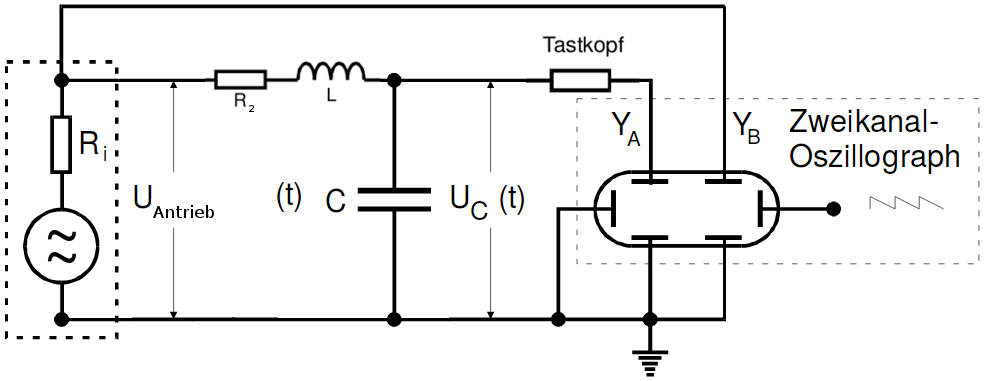
\includegraphics[width=\linewidth-150pt,height=\textheight-150pt,keepaspectratio]{content/Aufgabec.png}
         \caption{Schaltung zur Untersuchung der Resonanzeffekte und Phasenverschiebung zwischen $A_C$ und $A_{\text{Antrieb}}$ \cite{V354}.}
         \label{fig:Schalplanc}
       \end{figure}
 Die oben dargestellte Schaltskizze zeigt einen Versuchsaufbau zur Analyse eines
 angetriebenen $RCL$-Kreises. Die Messaperratur besteht im Kern aus einem
  $RCL$-Kreis in Reihenschaltung. Um diesen einer periodischen Spannung zu unterwerfen, wird ein
   Funktionsgenerator angeschlossen. Zur Betrachtung der Spannungsverläufe am
    Kondensator wird ein Zweikanaloszilloskop an diesem zugeschaltet. Um
     Störungen zu vermeiden wird die Spannung über einen hochohmigen Tastkopf abgenommen.
      Im späteren Versuchsverlauf wird auch der zweite Kanal des Oszilloskops verwendet.
